%!TEX root = ../../Master.tex
\subsection{ROS node}
Selve ROS noden der står for at køre vores program er meget simpel da alt kompleksitet er abstraheret væk i klasserne Camera og CrustCrawler, der henholdsvist står for at identificere klodser og flytte klodser. \\

Figur \ref{fig:node-flow} viser flowet i node programmet.
Programmet skal samle klodserne op og sortere dem efter farve.
Klodserne placeres til venstre og højre side af robotten, så de ikke længere er inden for vision programmets synsfelt. \\

Den første klods placeres altid til højre for robotten og herefter sker sorteringen.
Farven på de næste klodser sammenlignes med den første klods og hvis farverne er tæt nok på hinanden, sættes denne klods også til højre, ellers sættes den til venstre. \\

Alle farver og positioner registreres før robotten starter sin sortering.
Det betyder at hvis robotten fejler i at idetificere eller samle en klods op, bliver den liggende på bordet.
Derfor implementerede vi fejlhåntering ved at tage et nyt billede efter robotten er færdig, for at tjekke at den fik det hele med.
Hvis nye klodser identificeres starter robotten igen, indtil der ikke er flere klodser.
Denne løsning gør det også muligt at ligge flere klodser på bordet, og få disse klodser sorteret, efter robotten er startet.

\begin{figure}
	\centering
	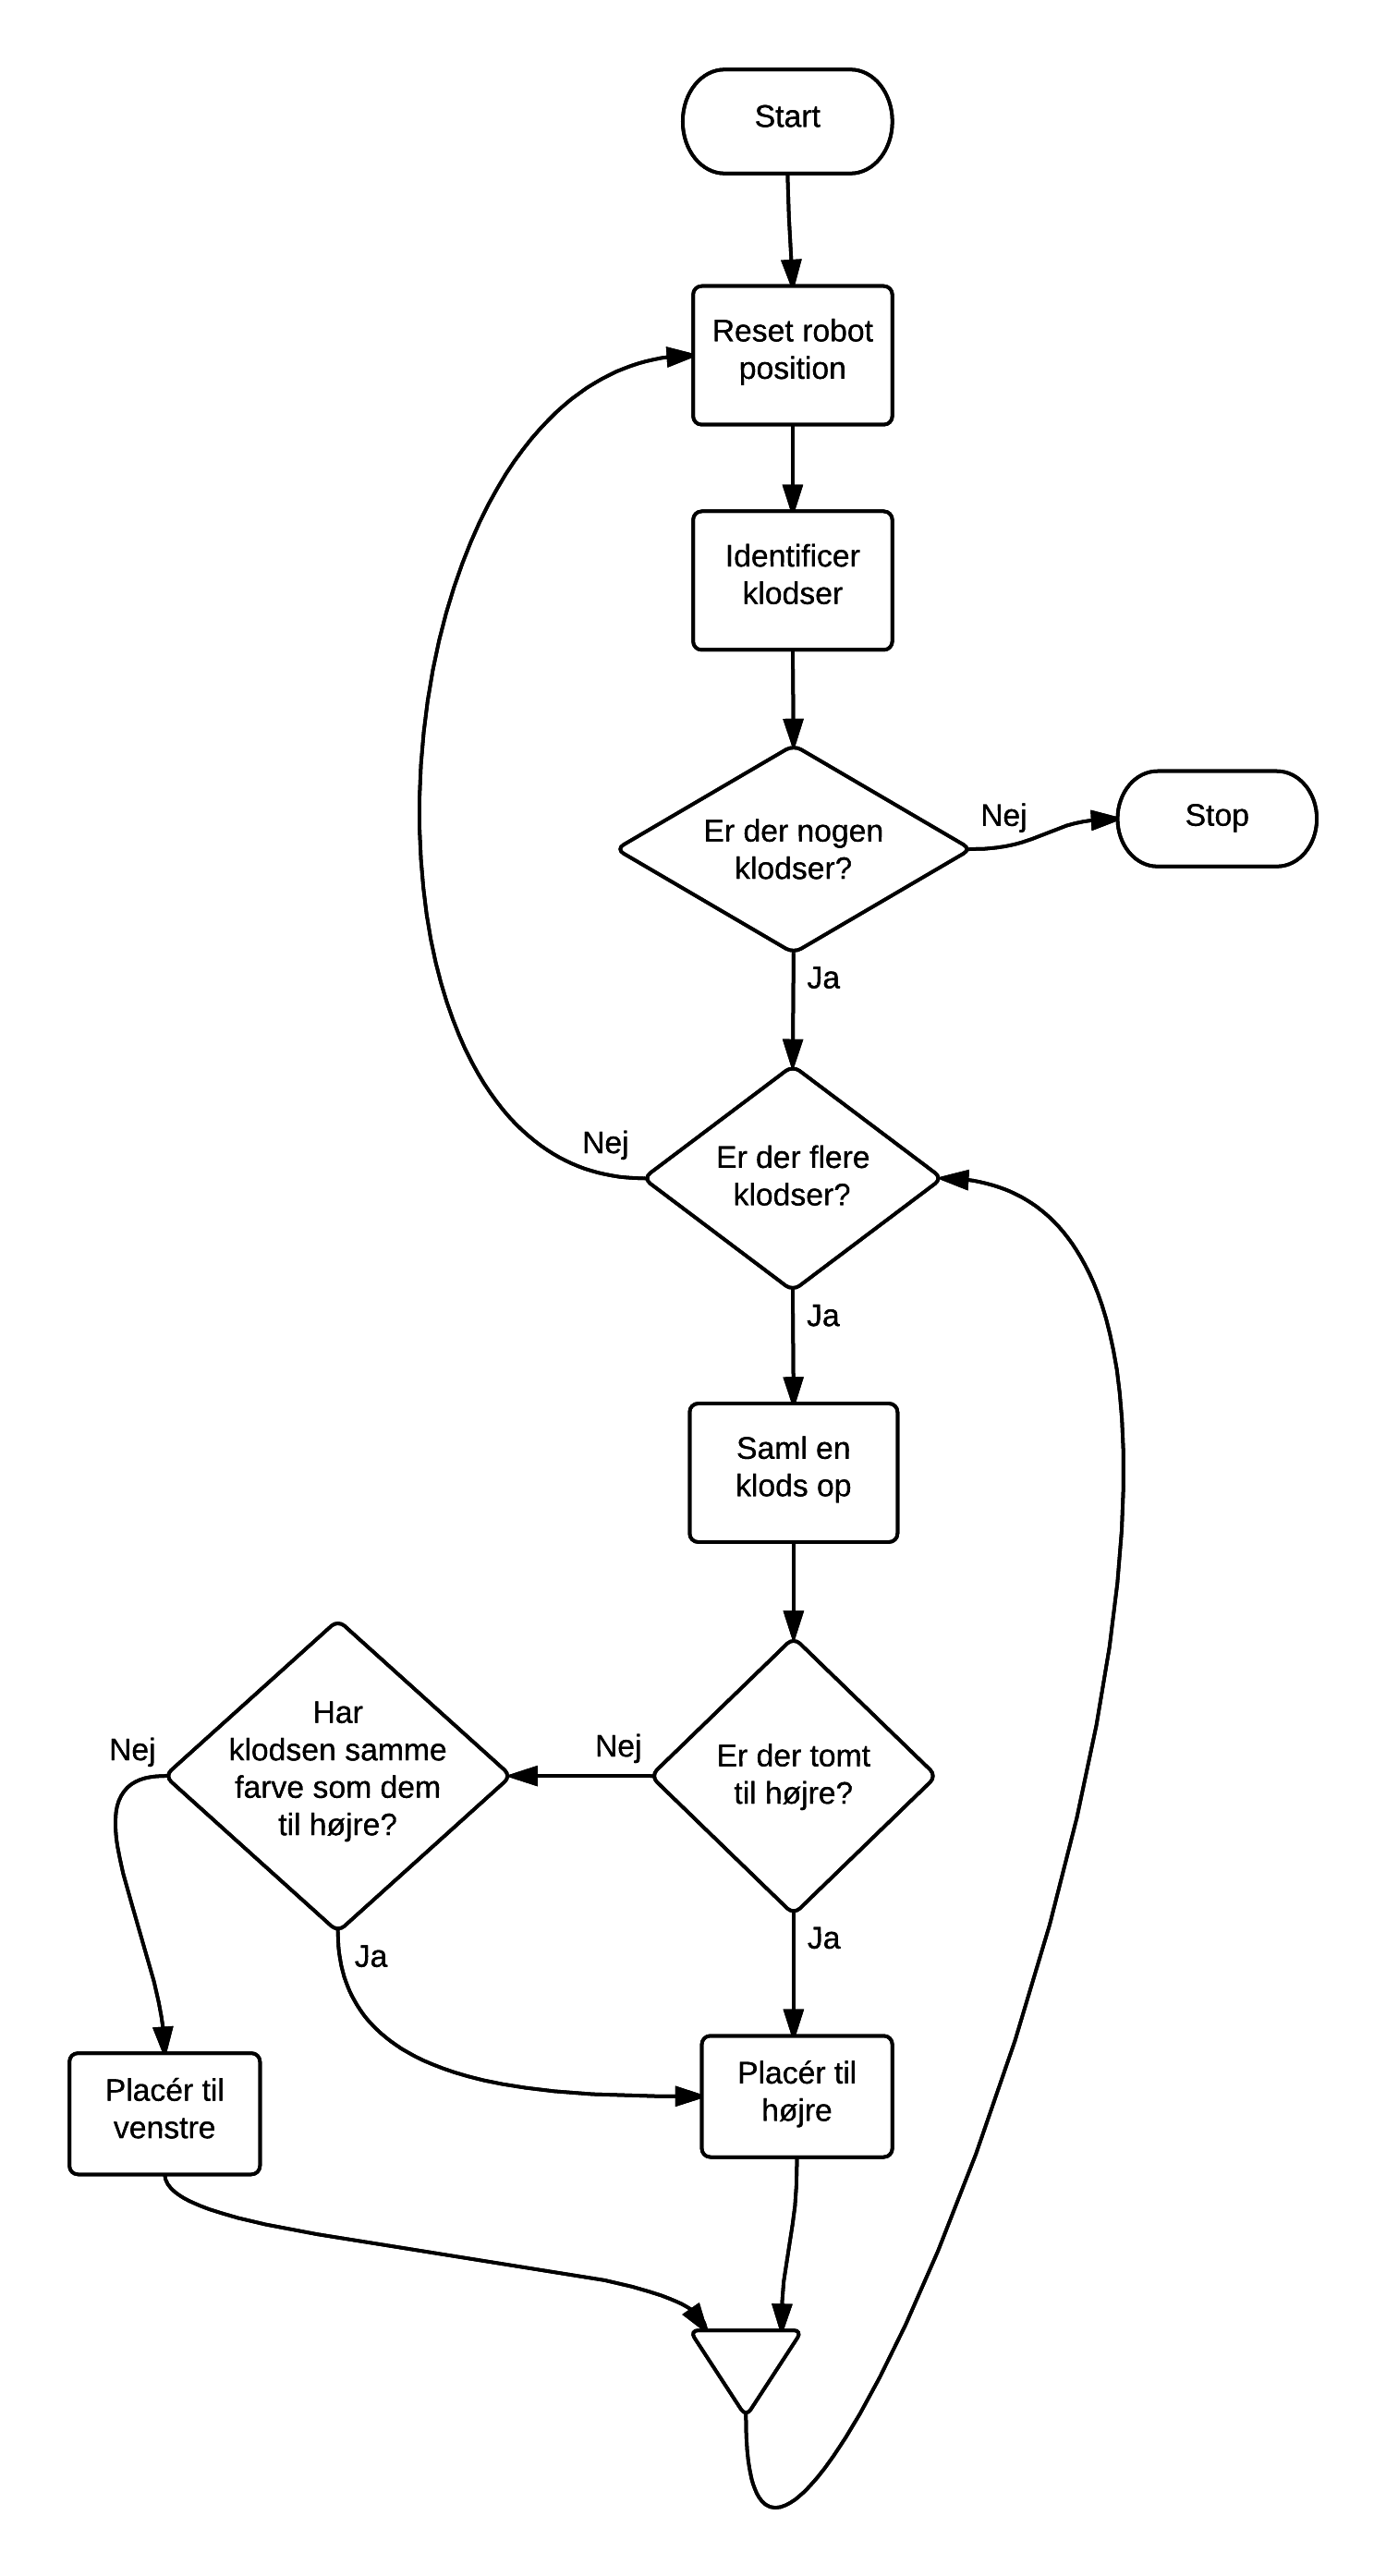
\includegraphics[scale=.7]{images/node-flow}
	\caption{Flowdiagram for ROS node}
	\label{fig:node-flow}
\end{figure}